\documentclass{article}

\usepackage{../tex/advi}
\usepackage{alltt}
\usepackage{color}
\usepackage{graphicx}

\begin{document}

\noindent
{\bf\Large Active dvi macros}\\

\noindent

\includegraphics[width=\textwidth]{../tex/bar.jpg.eps}

\section{Pause}

\begin{description}
\item[Syntax]  \verb!\pause!
\item[Effect] Stop the DVI command rendering at its occurrence.
\end{description}

\begin{minipage}[t]{0.5\textwidth}
\begin{alltt}
Please hit space!{\color{blue}\verb!\!pause}\verb!\\!
Ok, let's continue.
\end{alltt}
\end{minipage}
\begin{minipage}[t]{0.5\textwidth}
Please hit space!\\ \pause Ok, let's continue.
\end{minipage}

\section{Wait}

\begin{description}
\item[Syntax]  \verb!\wait{!{\em{sec}}\verb!}!
\item[Effect] Delay the DVI command rendering for {\em{sec}} seconds.
\item[Note] Due to the interval timer calls in the graphics library,
  the delay tends to be longer than the {\em{sec}} seconds.
\end{description}

\begin{minipage}[t]{0.5\textwidth}
\begin{alltt}
Let's animate a bit.\verb!\pause\\!
Un,{\color{blue}\verb!\wait{1.5}!}
Deux,{\color{blue}\verb!\wait{1.5}!}
Trois{\color{blue}\verb!\wait{1.5}!}!! 
\end{alltt}
\end{minipage}
\begin{minipage}[t]{0.5\textwidth}
Let's animate a bit.\pause\\
Un,\wait{1.5}
Deux,\wait{1.5}
Trois\wait{1.5}!! 
\end{minipage}

\section{Record and Play -- Color change}

\begin{description}
\item[Syntax]  \verb!\tag{!{\em{this}}\verb!}{!{\em{txt}}\verb!}!
\item[Effect] Associate the DVI commands correspond with {\em{txt}} to
  the Active dvi tag {\em{this}}.
\item[Note] This macro is used to change the color of {\em{txt}}
  later, with the combination of the \verb!\hilight! macro.
  The tag scope is restricted to the current page.
  By using the \verb!\tag{}{}! macro with the same tag name more than once,
  different parts of the page can be associated to the same tag.
\item[Bug] If the tagged text {\em{txt}} contains other tag related
 commands inside, they are ignored.
\end{description}

\begin{description}
\item[Syntax]  \verb!\hilight{!{\em{color}}\verb!}{!{\em{this}}\verb!}!
\item[Effect] Change the color of the texts associated to the tag {\em{this}}.
\item[Note] You need to use the style \verb!color.sty! from the
\verb"graphics" LaTeX package.
\end{description}

\begin{minipage}[t]{0.5\textwidth}
\begin{alltt}
{\color{blue}\verb!\tag{red}{Red}!}, 
{\color{blue}\verb!\tag{green}{Green}!} and 
{\color{blue}\verb!\tag{blue}{Blue}!} are
{\color{blue}\verb!\tag{red}{Rouge}!}, 
{\color{blue}\verb!\tag{green}{Vert}!} and 
{\color{blue}\verb!\tag{blue}{Bleu}!} in French.
Difficult to remember ?
Then, hit space!\verb!\pause!
{\color{blue}\verb!\hilight{red}{red}!}
{\color{blue}\verb!\hilight{green}{green}!}
{\color{blue}\verb!\hilight{blue}{blue}!}
\end{alltt}
\end{minipage}
\begin{minipage}[t]{0.5\textwidth}
\tag{red}{Red}, 
\tag{green}{Green} and 
\tag{blue}{Blue} are
\tag{red}{Rouge}, 
\tag{green}{Vert} and 
\tag{blue}{Bleu} in French.
Difficult to remember ? 
Then, hit space!\pause
\hilight{red}{red}
\hilight{green}{green}
\hilight{blue}{blue}
\end{minipage}
\noindent
Easy, no ? Hit space to continue!\pause

\section{Record and Play -- Hiding}

\begin{description}
\item[Syntax]  \verb!\hide{!{\em{this}}\verb!}{!{\em{txt}}\verb!}!
\item[Effect] The DVI commands are associated to the tag {\em{this}}
  as with the macro call \verb!\tag{!{\em{this}}\verb!}{!{\em{txt}}\verb!}!, 
  but the {\em{txt}} text argument is not rendered.
\item[Note] The hidden text can be displayed later by calling the
  \verb!\play! macro.
\item[Bug] If the tagged text {\em{txt}} contains other tag related
  commands inside, they are ignored.
\end{description}

\begin{alltt}
\verb!\begin{tabular}[t]{cccc}!
\verb!  One & !{\color{blue}\verb!\hide{tag2}{Two}!}\verb! & !{\color{blue}\verb!\hide{tag3}{Three}!}\verb! & Caml!{\color{blue}\verb!\hide{tag2}{s}!}\verb!\\!
\verb!  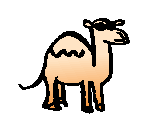
\includegraphics[width=0.1\textwidth]{../tex/caml.eps}&!
\verb!  !{\color{blue}\verb!\hide{tag2}{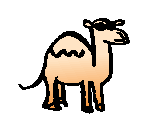
\includegraphics[width=0.1\textwidth]{../tex/caml.eps}!}\verb!}&!
\verb!  !{\color{blue}\verb!\hide{tag3}{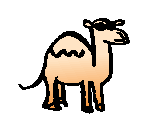
\includegraphics[width=0.1\textwidth]{../tex/caml.eps}!}\verb!}!
\verb!\end{tabular}!
\color{blue}\verb!\pause!
\verb!\play{tag2}!
\verb!\pause!
\verb!\play{tag3}!
\end{alltt}
\begin{tabular}[t]{cccc}
  One & \hide{tag2}{Two} & \hide{tag3}{Three} & Caml\hide{tag2}{s}\\
  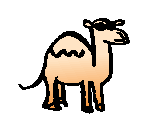
\includegraphics[width=0.1\textwidth]{../tex/caml.eps}&
  \hide{tag2}{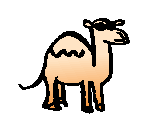
\includegraphics[width=0.1\textwidth]{../tex/caml.eps}}&
  \hide{tag3}{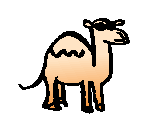
\includegraphics[width=0.1\textwidth]{../tex/caml.eps}}
\end{tabular}
\pause
\play{tag2}
\pause
\play{tag3}

\end{document}
